\documentclass[UTF8]{ctexart}
\usepackage{geometry, CJKutf8}
\geometry{margin=1.5cm, vmargin={0pt,1cm}}
\setlength{\topmargin}{-1cm}
\setlength{\paperheight}{29.7cm}
\setlength{\textheight}{25.3cm}


% useful packages.
\usepackage{amsfonts}
\usepackage{amsmath}
\usepackage{amssymb}
\usepackage{amsthm}
\usepackage{enumerate}
\usepackage{graphicx}
\usepackage{multicol}
\usepackage{fancyhdr}
\usepackage{layout}
\usepackage{listings}
\usepackage{float, caption}

\lstset{
    basicstyle=\ttfamily, basewidth=0.5em
}

% some common command
\newcommand{\dif}{\mathrm{d}}
\newcommand{\avg}[1]{\left\langle #1 \right\rangle}
\newcommand{\difFrac}[2]{\frac{\dif #1}{\dif #2}}
\newcommand{\pdfFrac}[2]{\frac{\partial #1}{\partial #2}}
\newcommand{\OFL}{\mathrm{OFL}}
\newcommand{\UFL}{\mathrm{UFL}}
\newcommand{\fl}{\mathrm{fl}}
\newcommand{\op}{\odot}
\newcommand{\Eabs}{E_{\mathrm{abs}}}
\newcommand{\Erel}{E_{\mathrm{rel}}}

\begin{document}

\pagestyle{fancy}
\fancyhead{}
\lhead{郭子昊, 3230104714}
\chead{数据结构与算法项目作业}
\rhead{Dec 8th, 2024}

\section{设计思路}
\indent 关于expression\_evaluator的设计思路:\\
\indent 我首先设计了一个类ExpressionEvaluator。
其中设置evaluator为类的公共借口,用来评估传入的中缀表达式;设置私有成员函数parseExpression用来解析加法和减法运算,
parseTerm用来解析乘法和除法运算,parseFactor用来解析数字和括号,parseNumber用来解析整数、小数和科学计数法,skipWhitespace用来跳过表达式中的空白字符。\\
\indent 关于main的设计思路:\\
\indent 首先要对输入表达式进行处理,通过初始化pos为0,调用 parseExpression 方法解析表达式并计算结果,调用skipWhitespace去掉空白字符,检查是否解析到了表达式的末尾,如果没有,抛出异常 "ILLEGAL"。\\
我利用parseExpression方法解析加法和减法运算,调用parseTerm解析第一个项,进入循环并跳过空白字符,并通过判断是否到达表达式末尾和当前字符op是否是$+$和$-$来结束循环,移动到下一个字符同理解析下一个项,并且根据op更新结果result。\\
\indent 再利用parseTerm方法解析乘法和除法运算,调用parseFactor解析第一个因子,进入循环并跳过空白字符,并通过判断是否到达表达式末尾和当前字符op是否是$*$和$/$来结束循环,移动到下一个字符同理解析下一个项,并且根据op更新结果result。\\
\indent 再利用parseFactor方法解析数字、正负号和括号。跳过空白字符,检查是否到达表达式末尾,如果是,抛出异常 "ILLEGAL";如果当前字符是左括号,解析括号内的表达式,并检查是否有匹配的右括号。
如果当前字符是$+$或 $-$,解析下一个因子,并根据符号返回正或负的因子值。否则,调用parseNumber方法解析数字。\\
\indent 接着利用parseNumber方法解析整数、小数和科学计数法。跳过空白字符,记录起始位置 start,检查是否有正负号。然后解析数字和小数点,如果有多个小数点,抛出异常 "ILLEGAL"。
然后解析科学计数法的指数部分,如果格式不正确,抛出异常 "ILLEGAL"。如果没有解析到任何数字,抛出异常 "ILLEGAL"。最后返回解析的数字。\\
最后利用skipWhitespace方法跳过空白字符。\\




\section{测试的结果}

测试结果一切正常。详细的结果见照片。\\

\begin{figure}[h]
    \centering
    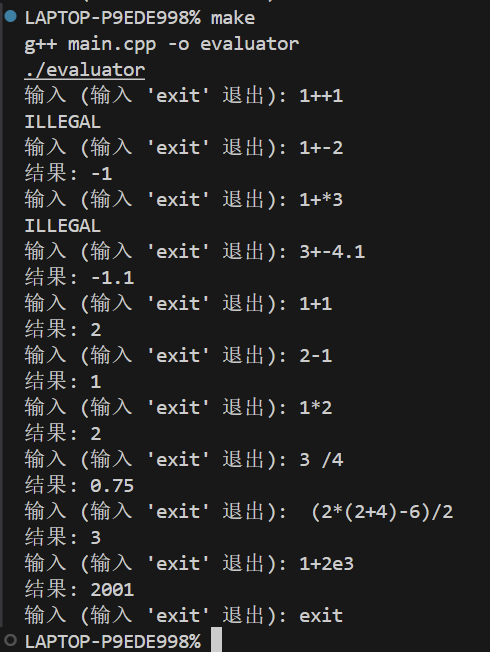
\includegraphics[width=0.5\textwidth]{./ceshi.png}
    \caption{Test}
    \label{fig:photo}
\end{figure}



\end{document}

%%% Local Variables: 
%%% mode: latex
%%% TeX-master: t
%%% End: 
